\documentclass[12pt, a4paper, lithuanian, final]{article}

\usepackage{hyperref}
\usepackage{graphicx}
\usepackage{float}
\usepackage{placeins}
\usepackage{gensymb}
\usepackage{xcolor}
\usepackage{listings}
\usepackage{amsmath}
\usepackage{textgreek}
\usepackage{mathtools}
\usepackage[obeyFinal]{easy-todo}
\usepackage[utf8]{inputenc}
\def\LTfontencoding{L7x}
\usepackage[\LTfontencoding]{fontenc}
\usepackage[lithuanian]{babel}
%\usepackage{times}

%\renewcommand{\sfdefault}{uhv}
%\renewcommand{\rmdefault}{utm}
%\renewcommand{\ttdefault}{ucr}

\usepackage{VUMIF}

%Kodo highlitinimo configas
\lstset{basicstyle=\ttfamily,
	showstringspaces=false,
	commentstyle=\color{red},
	keywordstyle=\color{blue}
	}


% Titulinio puslapio reikalai
\vumifdept{Programų sistemų katedra}
\vumifpaper{Bakalauro baigiamasis darbas}
\title{Autonominis ketursraigčio skrydžio valdymas\\Autonomous Control of Quadcopter Flight}
\author{
    4 kurso 1 grupės studentas \\
    Rytis Karpuška
}

\supervisor{Irus Grinis, lekt.}
\reviewer{Vytautas Valaitis, lekt.}
\date{Vilnius 2015}


\begin{document}

%titulinis ir turinys
\maketitle

\vumifsectionnonum{Santrauka}
Šio darbo metu buvo sukurti ir išbandyti algoritmai ketursraigčio autonominiam skrydžiui palaikyti, bandymus atliekant su realiu ketursraigčiu.
Ši užduotis buvo išskaidyta į tris dalis: kampinės pozicijos įvertinimas, kampinės pozicijos valdymas bei abosliučios pozicijos valdymas.
Kampinė pozicija yra skaičiuojama pasitelkiant kvaternionus, šitaip efektyviai atliekant skaičiavimus įterptinės sistemos aplinkoje bei išvengiant užrakinimo (ang.: \textit{gimbal lock}) problemos.
Kampinės pozicijos valdymas atliekamas naudojant du PID nuosekliai sujungtus valdiklius.
O absoliuti pozicija valdoma atviro-ciklo (ang.: \textit{open-loop}) valdiklio, kuriam yra saugoma tam tikrų kampinių pozicijų lentelė ir jos duomenys yra persiunčiami kampinės pozicijos valdikliams tam tikru laiko momentu.

\paragraph{Raktiniai žodžiai} Ketursraigtis, inercinis matavimo įrenginys, kvaternionai, kampinė pozicija, PID, uždaro-ciklo valdiklis, atviro-ciklo valdiklis, autonominis



\vumifsectionnonum{Summary}
During this thesis algorithms for autonomous quadcopter control has been developed and tested in a real environment.
Autonomus control of quadcopter has been divided into three parts: angular position estimation, angular position control and absolute position control.
Angular position estimation is being performed using quaternions in order to exrpess 3D rotations efficiently and to avoid gimbal lock problem.
Angular position control is achieved using two PID controllers connected in series.
And absoulte position control is achieved by using open-loop controller where a table of certain angular positions are saved and at apropriate times sent to the angular position controller algorithms.

\paragraph{Keywords} Quadcopter, inertial measurement unit, quaternion, attitude, PID, closed-loop controller, open-loop controller, autonomous




\newpage
\tableofcontents


\vumifsectionnonum{Įvadas}

Ketursraigčiai per keletą paskutinių metų pradėjo stipiriai populiarėti, ypač akadėminėje ir mėgėjų aplinkoje.
Tačiau jie yra ir gali būti taikomi labai plačiose srityse, pradedant nuo pirmo-asmens vaizdo (ang.: \textit{first-person-view}) įrenginių mėgėjų skraidymui, įvairių renginių ar įvykių filmavimu ir baigiant vaistų pristatymu sunkiai prieinamiems ligoniams ar
gelbėjimo ir paieškos tipo operacijose.
Tobulėjančios akumuliatorių bei elektrinių variklių technologijos leidžia išlaikyti ketursraigtį ore vis ilgiau ir užkrauti vis sunkesnius krovinius.
Tačiau ketursraigčių valdymas yra perdaug sudėtingas, kad pilotas galėtų vadyti ketursraigčio skrydį tiesiogiai, todėl elektroninių sistemų pagalba yra būtina.
Ši sistema priima paprastesnes žmogui komandas iš piloto, pavyzdžiui "`skristi pirmyn"', "`skristi šonan"' ir t.t. ir paskui paverčia jas elektriniais variklių signalais.
Šio darbo tikslas yra sukurti, suprogramuoti ir išbandyti tokią ketursraigčio skrydžio valdymo sistemą.
Tam buvo surinktas vidutinio dydžio ketursraigtis, ir paruošta elektroninė įranga.

\begin{figure}[H]
\begin{center}
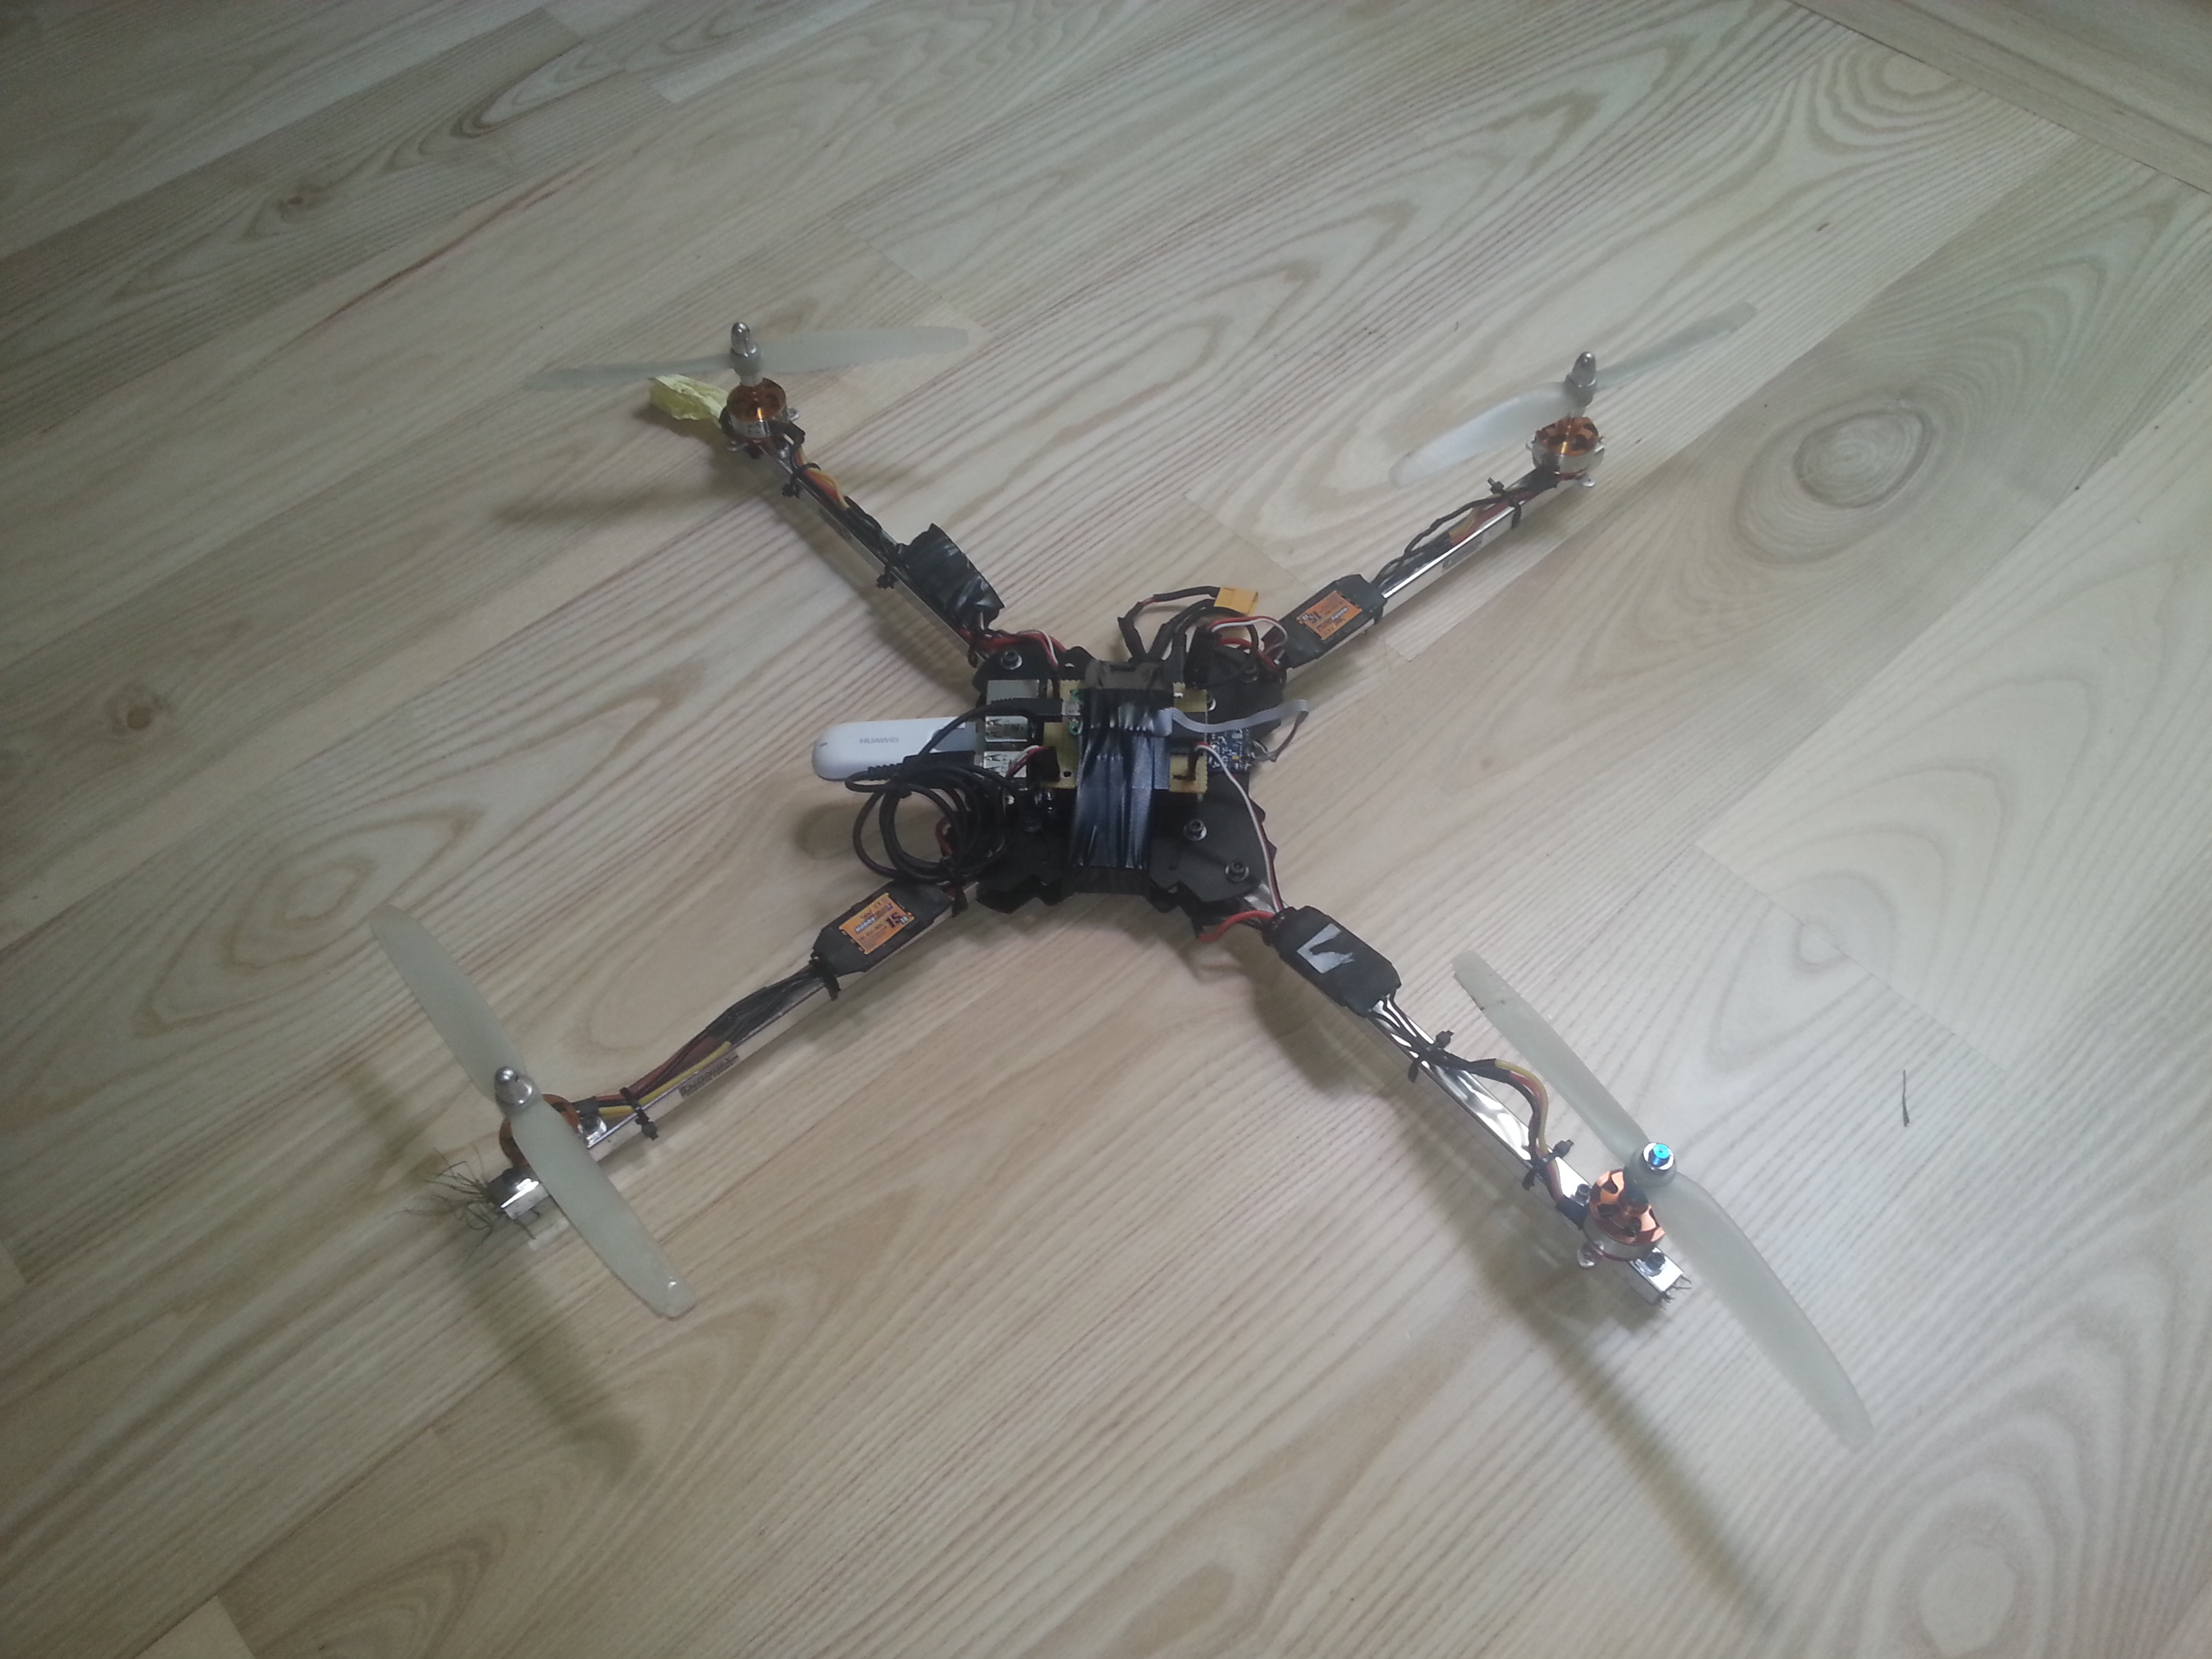
\includegraphics[width=0.75\textwidth]{img/quad.jpg}
\caption{Ketursraigtis.}
\end{center}
\end{figure}


\paragraph{Testavimo aplinka}

Ketursraigčio valdymo algoritmų kūrimas yra labai apsunkinamas, dėl sudėtingų testavimo sąlygų.
Neištestavus pakeitimų kode negalima leisti ketursraigčiui laisvai skristi, nes klaidos atveju, ketursraigtis gali atsitrenkti į kliūtį, sulaužyti savo dalis, ar blogiausiu atveju, dėl daugiau kaip 10,000 sūkių per minutę besisukančių propelerių -- stipriai sužeisti aplink esančius žmones ar gyvūnus.
Tačiau duomenų surinkimas apie algoritmų darbą negali įvykti, kol šie algoritmai nebuvo įdarbinti realioje aplinkoje, o dėl sudėtingos ketursraigčių dinamikos bei aerodinamikos -- realistiškos simuliacijos atlikimas yra perdaug sudėtinga užduotis.
Susiduriama su "`vištos ir kiaušinio"' problema, algoritmai negali būti tobulinami, kol jie nebuvo paleisti darbui, bet algoritmų negalima paleisti darbui, kol jie neištobulinti.

Šiai problemai spręsti buvo sumontuotas specialus stendas, apribojantis ketursraigčio judėjimo laisvę.
Stendas susideda iš pakankamai sunkaus stovo, kurio ketursraigtis negalėtų nuversti ar pakelti, netgi generuodamas maksimalią traukos jėgą.
Toliau yra mechanismas užfiksuojantis ketursraigtį stove taip, kad ketursraigtis galėtų suktis tiktai apie vieną ašį.
Konkrečiu atveju buvo ištiesta plieninė styga, išilgai kurios buvo tvirtinamas ketursraigtis $X$ arba $Y$ ašimi.

\begin{figure}[H]
\begin{center}
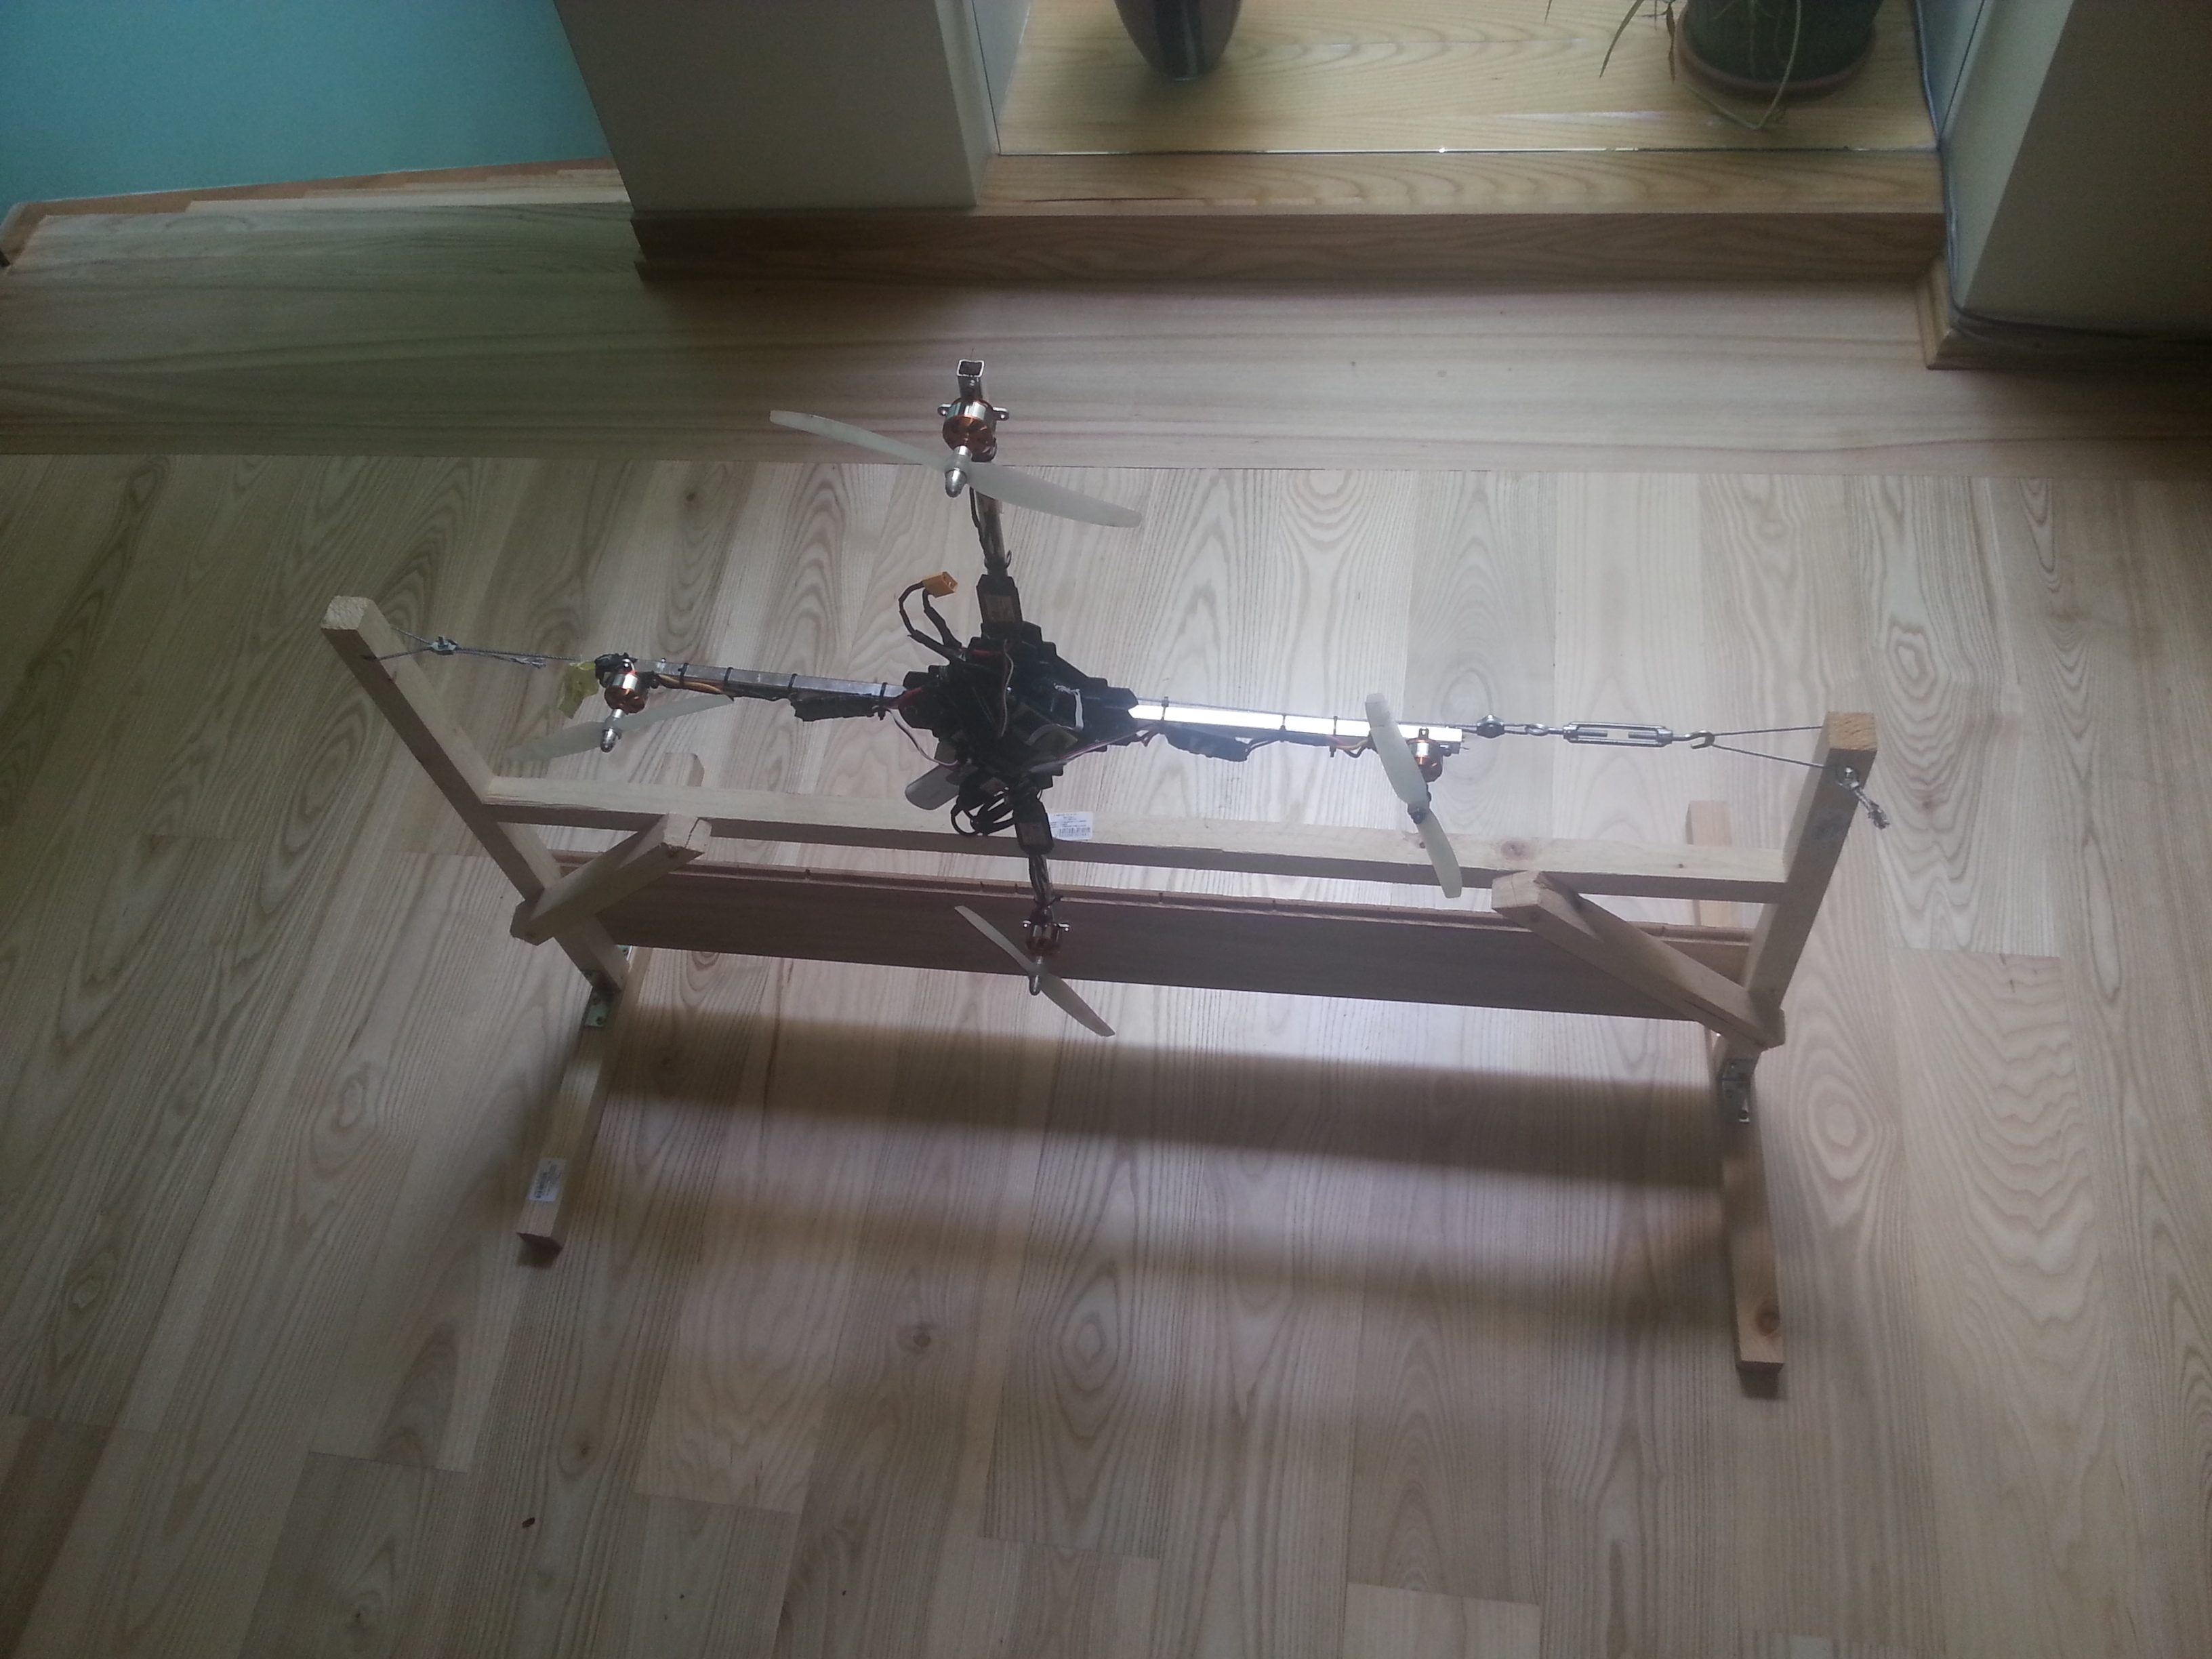
\includegraphics[width=0.75\textwidth]{img/frame.jpg}
\caption{Ketursraigčio stendas.}
\end{center}
\end{figure}



Šis stendas išsprendė testavimo sudėtingumo problemą ir leido algoritmų testavimo metu prijungti įvairius komunikacijos ar galios laidus prie ketursraigčio, tad supaprastėjo duomenų kaupimas, derinimas, taip pat galima buvo atlikti testavimus su išoriniu maitinimo šaltiniu vietoj baterijų, o tai leido sutaupyti laiko, dėl ilgo baterijos krovimosi laiko.




\paragraph{Literatūros apžvalga}

Paskutiniu metu ketursaigčių valdymo sistemos irgi susilaukė palyginus nemažai mokslininkų ir tyrėjų dėmesio.

\cite{abyarjoo2015implementing} pateikia kampinės padėties skaičiavimus pagal inercinius ir magnetinius sensorius, paaiškina sensorių savybes, ir pasiūlo oilerio kampais grystą kampinės pozicijos įvertinimo būdą.
Taip pat sumodeliuoja kalmano filtrą giroskopo dreifavimo problemai spręsti.


Straipsnyje \cite{kumar2004estimation} autoriai pateikia sensorių modelį, bei kalibravimo procedūras, nors jų IMU nebuvo taikomas ketursraigčiuose.
Taip pat pasiūlomas kampinės padėties įvertinimo algoritmas naudojant kalmano filtrą su statiniu stiprinimo koeficientu.


Papildomasis (ang.: \textit{complementary}) filtras panaudojamas \cite{euston2008complementary} skaičiuojant kampinę poziciją fiksuoto sparno lėktuvui.
Atlikti tyrimai parodo akselerometro triukšmo lygius, bei filtravimo būdus.

Teorinė ketursraigčio valdymo sistema analizuojama \cite{gibiansky2010quadcopter}, kartu su fizikinių ketursraigčio modeliu, bei atliekama simuliacija.
\cite{gibiansky2010quadcopter} buvo remtasi išvedant fizikinį modelį šiame darbe.

\cite{magnussen2011modeling} pateikia valdymo sistemą sistemą valdomą FPGA valdiklio.

Nors FPGA ir gali pasiūlyti greitesnį duomenų apdorojimą, tačiau \cite{magnussen2011modeling} kontroleris dirbo 100Hz dažniu, tuo tarpu, kai šiame darbe atnaujinimai vykdomi 500Hz dažniu, nors ir naudojamas ne FPGA, bet ARM procesorius.
Taip pat \cite{magnussen2011modeling} naudoja oilerio kampus kampinės pozicijos skaičiavimui, todėl kampinė pozicija potencialiai gali užsirakinti (ang.: "`gimbal lock"').
Skrydžio kampinės padėties valdymo algoritmui buvo naudojamas P valdiklis ir kampinės padėties greičio kompensavimas, tačiau išvadose rašoma, kad ore ketursraigtis negalėjo išsilaikyti.
Tačiau \cite{magnussen2011modeling} atliko labai naudingus ESC tiesiškumo, traukos bei sukimo momento priklausomybių empirinius testus.





\section{Ketursraigčio techninė įranga}
\label{skyr-hardware}
Įprasto ketursraigčio techninė struktūra yra palyginus lengvai suprojektuojama bei pagaminama, tačiau to negalima pasakyti apie programinę įrangą, bei algoritmus valdančius skrydį.



\subsection{Rėmas, varikliai ir propeleriai}
Ketursraigtis susideda iš "`X"' formos rėmo, kurio galuose yra po elektrinį bešepetėlinį variklį su propeleriu.
Priešingai nei įprastuose sraigtasparniuose, šių propelerių atakos kampas nėra reguliuojamas, o tai leidžia stipriai supaprastinti skraidyklės techninę struktūrą ir atsisakyti sudėtingų mechaninių dalių.
Varikliai skirstomi į dvi grupes iš kurių viena sukasi pagal laikrodžio rodyklę, kita -- prieš laikrodžio rodyklę.
Šių variklių sukimosi greitis yra reguliuojamas siekiant išgauti tinkamą sukamąją bei keliamąją jėgas.

\begin{figure}[H]
\begin{center}
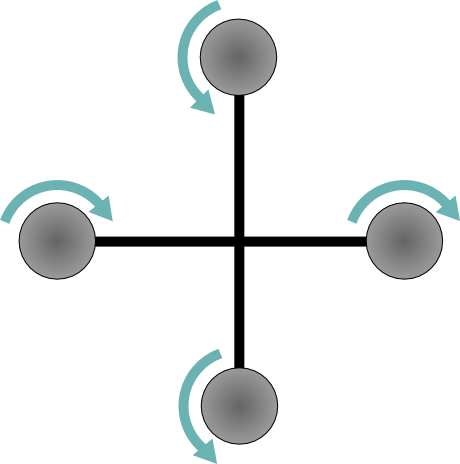
\includegraphics[width=0.5\textwidth]{img/rotor-direction.png}
\caption{Ketursraigčio rėmo ir variklių išdėstymas. Jų sukimosi kryptys.}
\end{center}
\end{figure}

Šio darbo tikslams pasiekti buvo nupirktas "`HobbyKing x525"' 600 mm skersmens rėmas, pagamintas iš aliuminio ir stiklo pluošto.
Taip pat elektriniai bešepetėliniai 160 W galios varikliai "`Turnigy D2822"' ir 8 colių ilgio, bei 4 laipsnių atakos kampo propeleriai.


\subsection{Valdymo elektronika}
Stabilaus skrydžio išlaikymas ketursraigtyje yra per sudėtinga užduotis žmogui (pilotui) todėl pasitelkiama pagalbinė elektronika palengvinanti ketursraigčio valdymą.

Valdymo elektronikai išskiriami tokie uždaviniai:
\begin{itemize}
	\item skrydžio stabilizavimas bei kontrolė;
	\item ryšio su pilotu arba valdančia sistema palaikymas;
	\item galios signalų, reikalingų varikliams, generavimas.
\end{itemize}

\paragraph{Skrydžio stabilizavimas bei kontrolė}
Skrydžio stabilizavimui bei kontrolei atlikti naudojami sensoriai pagal kurių duomenis yra paskaičiuojami kokių korekcinių veiksmų reikia imtis norint įgyvendinti piloto ar valdančios sistemos komandas.
Išskiriami svarbiausi parametrai yra tikslumas bei greitis.

Atsižvelgiant į rekalavimus šiems parametrams, buvo parinktas kompanijos "`STMicroelectronics"' procesorius "`STM32F401"' bei kompanijos "`InvenSense"' sensorius "`MPU6050"'

\paragraph{Ryšio su pilotu arba valdančia sistema palaikymas}
Ryšio palaikymas parametrizuojamas pagal duomenų persiuntimo greitį ir uždelsimą, bei veikimo ribas.
Ketursaigčio atveju persiunčami duomenys yra tik valdymo signalai iš piloto arba valdančios sistemos, todėl buvo pasirinktas GSM ryšys.
Taip pat "`Raspberry pi"' kompiuteris su "`Linux"' operacine sistema atlikdavo viską kas reikalinga GSM ryšiui palaikyti.

\paragraph{Galios signalų generavimas}
Bešepetėliniai varikliai reikalauja trijų galios signalų jų sukimuisi palaikyti.
Šiam tiklui buvo nupirkti 18 A elektroniniai greičio valdikliai galintys suvaldyti apie 200 W galios, tad puikiai tinkantys 160 W galios varikliams.

\begin{figure}[H]
\begin{center}
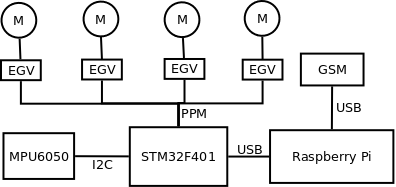
\includegraphics[width=0.5\textwidth]{img/elektronikosSchema.png}
\caption{Ketursraigčio elektronikos sudedamųjų dalių schema.}
\end{center}
\end{figure}




\section{Matematinis skrydžio modelis}
\label{skyr-model}



\subsection{Lokalioji ir globalioji koordinačių sistemos}
Pravartu apibrėžti lokaliają ir globaliąją koordinačių sistemas, kuriose bus nagrinėjama ketursraigčio dinamika.
Lokaliojoje koordinačių sistemoje $X$ ir $Y$ ašis yra sulygiuota su ketursraigčio rėmo strypais, kur $X$ rodo pirmojo variklio kryptimi, $Y$ - antrojo.
Globalioji sistema yra susieta su žemės gravitaciniu lauku, ir toje sistemoje gravitacinio lauko vektorius nukreiptas priešinga $Z$ ašiai kryptimi.

\begin{figure}[H]
\begin{center}
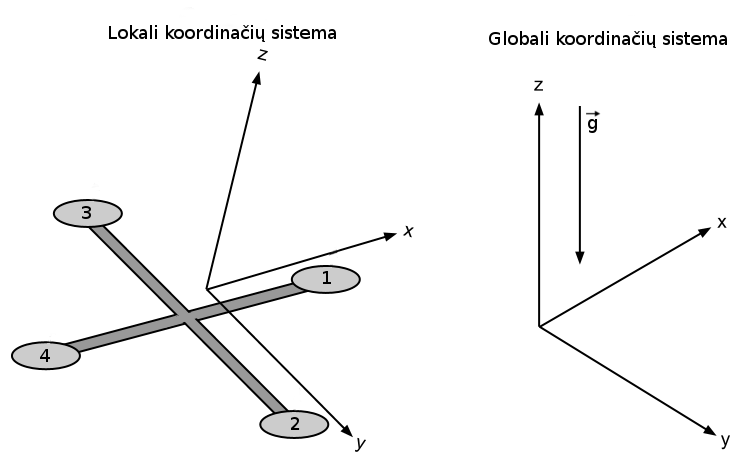
\includegraphics[width=1.0\textwidth]{img/Quadcopter_Coordinates.png}
\caption{Lokalioji ir globalioji koordinačių sistemos palyginimas.}
\end{center}
\end{figure}


Konvertavimas tarp šių koordinačių sistemų bus vykdomas kvaternionų pagalba (žr.: \ref{subskyr-quaternion}):

\begin{equation}
	q_{l} = q_{p} * q_{g} * q_{p}^{-1}
\end{equation}

ir į priešingą pusę:

\begin{equation}
	q_{g} = q_{p}^{-1} * q_{l} * q_{p}
\end{equation}

Čia $q_{g}$ -- tašką arba vektorių globaliojoje koordinačių sistemoje atvaizduojantis kvaternionas, $q_{l}$ -- tašką arba vektorių lokaliojoje koordinačių sistemoje atvaizduojantis kvaternionas, $q_{p}$ -- kampinės pozicijos kvaternionas (žr.: \ref{subskyr-quaternion}).





\subsection{Keliamoji jėga}

Ketursaigtis sukuria keliamąją jėgą priversdamas judėti orą žemyn.
Kadangi naudojami nekintamo atakos kampo propeleriai, keliamoji jėga reguliuojama valdant propelerių sukimosi greitį.
pagal \cite{gibiansky2010quadcopter,magnussen2011modeling} keliamoji jėga gali būti apskaičiuota:
\begin{equation}
	T = C * \omega^2
\end{equation}

Kur $T$ yra keliamoji jėga niutonais vienam varikliui, $C$ yra konstanta priklausanti tik nuo propelerio nekintamų savybių, o $\omega$ yra variklių sukimosi greitis.

Taip pat galime apskaičiuoti bendrąją keliamąją jėgą visiems varikliams.

\begin{equation}
	T = \left[
		\begin{array}{c}
			C_{1} * \omega_{1}^2 - C_{4} * \omega_{4}^2 \\
			C_{2} * \omega_{2}^2 - C_{3} * \omega_{3}^2\\
			\displaystyle\sum_{i=1}^{4} C_i * \omega_i^2
		\end{array}
	\right]
\end{equation}

Šiuo atveju $T$ yra keliamosios galios vektorius lokaliojoje koordinačių sistemoje.
Verta pastebėti, kad esant nevienodiems $\omega_{1}, \omega_{4}$ arba $\omega_{2}, \omega_{3}$ sukuriama jėga sukanti ketursraigtį apie jo lokalią $Y$ arba $X$ ašį atitinkamai.

O skaičiuojant globaliojoje koordinačių sistemoje:

\begin{equation}
q_{tl} = \left[
		\begin{array}{c}
			0\\
			T_x\\
			T_y\\
			T_z\\
		\end{array}
		\right]
\end{equation}
\begin{equation}
	q_{tg} = q_{p}^{-1} * q_{tl} * q_{p}
\end{equation}
\begin{equation}
	T_g = \left[
		\begin{array}{c}
			q_{tg_x} \\
			q_{tg_y} \\
			q_{tg_z}
		\end{array}
	\right]
\end{equation}

Čia $q_{tl}$ yra kvaternionas, reprezentuojantis keliamosios jėgos vektorių lokaliojoje koordinačių sistemoje, $q_{p}$ kvaternionas reprezentuojantis pasukimą nuo globaliosios iki lokaliosios koordinačių sistemos (žr.: \ref{skyr-attitude}), $q_{tg}$ -- keliamosios jėgos vektorių atvaizduojantis kvaternionas globaliojoje koordinačių sistemoje, $T_g$ -- keliamosios jėgos vektorius globaliojoje koordinačių sistemoje.





\subsection{Sukamoji jėga}

Besisukant propeleriams oro trintis į mentes sukelia papildomą jėgą, kuri veikia ketursraigčio rėmą.
Kiekvienam iš variklių ši jėga yra nukreipta priešinga kryptimi nei sukasi variklis.
Norint išvengti nevaldomo ketursraigčio sukimosi, parenkami du propeleriai skirti suktis pagal laikrodžio rodyklę ir du propeleriai skirti suktis prieš laikrodžio rodyklę, varikliai sujungiami taip, kad jų sukimosi kryptis atitiktų propelerį ir oro srautas būtų nukreiptas žemyn.
Konkrečiu atveju varikliai 1 ir 4 sukasi prieš laikrodžio rodyklę, o varikliai 2 ir 3 -- pagal.
Šitaip vienos krypties jėga kompensuoja kitą ir tampa įmanomas skrydis be sukimosi apie $Z$ ašį lokalioje koordinačių sistemoje.

Šią jėgą modeliuosime tiesiškai priklausančią nuo sukimosi greičio:
\begin{equation}
	F_{tq} = -\omega * C
\end{equation}

Čia $C$ yra konstata priklausanti tik nuo propelerio savybių. Sukamoji jėga yra sukeliama oro pasipriešinimo, todėl ji yra priešinga judėjimo krypčiai $\omega$.


\begin{figure}[H]
\begin{center}
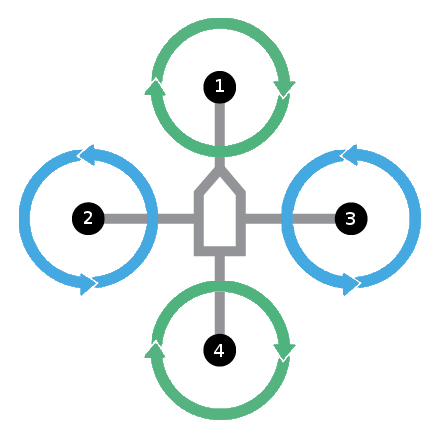
\includegraphics[width=0.6\textwidth]{img/quadcopter-torque.png}
\caption{Jėgos sukeliamos dėl oro trinties į propelerius.}
\end{center}
\end{figure}

Verta pastebėti, kad varikliai skaidomi grupėmis pagal sukimosi kryptį. Tos pačios sukimosi krypties variklis sukuria tos pačios krypties sukamąją jėgą, tik centras kitoje vietoje. Tačiau rėmo atžvilgiu šias grupes galima nagrinėti kaip vieną jėga.
Tokiu atveju turime dvi jėgas priešingų krypčių (žr.: pav. \ref{pav-grouped-forces}).

\begin{figure}[H]
\begin{center}
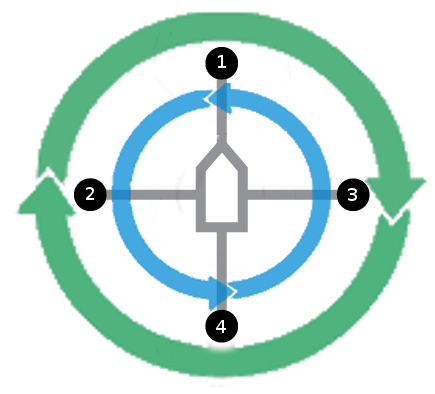
\includegraphics[width=0.75\textwidth]{img/quadcopter-torque-grouped.png}
\caption{Jėgos sukeliamos dėl oro trinties į propelerius.}
\label{pav-grouped-forces}
\end{center}
\end{figure}

Šiuo atveju vidinės rodyklės rodo 2 ir 3 variklių sukamąsias jėgas, o išorinės -- 1 ir 4 (žr.: pav. \ref{pav-grouped-forces}).
Verta pastebėti, kad rodyklių storis nėra susijęs su jėgos dydžiu.

Sukamosios jėgos neturi vieningos krypties, kuri nepriklausytų nuo stebėjimo pozicijos, todėl ji bus išreikšta ne vektorine forma, taigi nagrinėsime sukamosios jėgos dydį ties varikliais.
Taip pat, sakysime, kad jėga yra teigiama kai sukamasi apie lokalią $Z$ ašį pagal laikrodžio rodyklę.
Tada gauname, kad sukamoji jėga:
\begin{equation}
	F_{tq_{1,4}} = C * (\omega_{1} + \omega_{4})
\end{equation}
\begin{equation}
	F_{tq_{2,3}} = -C * (\omega_{2} + \omega_{3})
\end{equation}

Ir bendra jėga:
\begin{equation}
	F_{tq} = F_{tq_{1,4}} - F_{tq_{2,3}} = C * (\omega_{1} - \omega_{2} - \omega_{3} + \omega_{4})
\end{equation}

Šias jėgų kryptis atitinkamai galime pasukti priešingu kvaternionu $q_{p}$, ir gausime jėgą globaliojoje koordinačių sistemoje.
Verta pastebėti, kad šių jėgų kryptys visada bus lygiagračios su propelerių plokštuma.

\subsection{Bendras judėjimo modelis}

Ketursraigčio skrydžio judėjimui apibrėžti reikia įsivesti gravitacijos kryptį.

\begin{equation}
	g_{g} =  \left[
		\begin{array}{c}
			0 \\
			0 \\
			-9.8
		\end{array}
	\right]
\end{equation}

$g_{g}$ yra apibrėžtas globalioje koordinačių sistemoje.

Tuomet bendra jėga veikianti ketursraigtį:

\begin{equation}
	F_{g} = T_{g} - m*g_{g}
\end{equation}

Čia $m$  yra ketusraigčio bendra masė.

Toliau pagal antrąjį Niutono dėsnį:
\begin{equation}
	a_{g} = \dfrac{F_{g}}{m}
\end{equation}

kur $a$ yra pagreičio vektorius globalioje koordinačių sistemoje.

Toliau randamas greičio bei pozicijos priklausomybė nuo nykstamai mažo laiko pokyčio $\Delta$ t:
\begin{equation}
	v_{g} = a_{g} * \Delta t
\end{equation}
\begin{equation}
	x_{g} = a_{g} * \Delta t ^2
\end{equation}

Tais pačiais principais randama ir kampinė padėtis.







\section{Kampinės padėties skaičiavimas}
\label{skyr-attitude}

Ketursraigčio valdymo algoritmai yra tiesiogiai priklausomi nuo kampinės padėties, bet nėra sensorių leidžiančių tai išmatuoti tiesiogiai, todėl šiame skyrelyje apibūdinami sukurti principai, pagal kuriuos yra skaičiuojama ketursraigčio kampinė pozicija globaliosios koordinačių sistemos atžvilgiu.

Ketursraigčių kampinės padėties skaičiavimui buvo parinkta matematinė skaičiavimo sistema vadinama kvaternionais.
Šioje sistemoje trimačiai posūkiai gali būti atvaizduoti labai efektyviai ir patogiai.

\subsection{Kvaternionai}
\label{subskyr-quaternion}

Kvaternionai matematikoje yra skaičių sistema, kuri išplėčia įprastus kompleksinius skaičius.
Kvaternionas yra vektorius:

\begin{equation}
	q = \left[
		\begin{array}{c}
			w \\
			i \\
			j \\
			k
		\end{array}
	\right]
\end{equation}

kur $w$ yra sveikoji dalis, o $i$, $j$, $k$, yra menamosios.


Menamosios dalys tarpusavyje siejamos pagal:
\begin{equation}
	i^2 = j^2 = k^2 = ijk = -1
\end{equation}

Dauginimui kiekvieno elemento su kiekvienu naudojamas toks sąryšis:

\begin{center}
\begin{tabular}{ | c | c | c | c | c | }
	\hline
	\textbf{*} & \textbf{1} & \textbf{i} & \textbf{j} & \textbf{k} \\
	\hline
	\textbf{1} & 1 & i & j & k \\
	\hline
	\textbf{i} & i & -1 & k & -j \\
	\hline
	\textbf{j} & j & -k & -1 & i \\
	\hline
	\textbf{k} & k & j & -i & -1 \\
	\hline
\end{tabular}
\end{center}

Įprastas kvaternionas užrašomas kaip šių elementų suma:

\begin{equation}
	q = w + xi + yj + zk
\end{equation}

kur $w$, $x$, $y$, $z$ yra realioji skaičiai, o $i$, $j$, $k$ yra menamosios kvaterniono dalys.

Šiame darbe kvaternionai bus nagrinėjami naudojant vektorine forma:

\begin{equation}
	q = \left[
		\begin{array}{c}
			w \\
			xi \\
			yj \\
			zk
		\end{array}
	\right]
\end{equation}

Šio vektoriaus atskiras komponentes bus žymimos $q_w$, $q_x$, $q_y$, $q_z$.


\paragraph{Daugyba}

Kvaternionų daugyba atliekama pagal Hamiltono taisykles:

TODO sužiūrėti newlinenus
\begin{equation}
	q_1 * q_2 = \left[ w_1, x_1 i_1, y_1j_1, z_1k_1 \right] * \left[ w_1, x_1 i_1, y_1j_1, z_1k_1 \right] = \\
	q_1 * q_2 = \left[
		\begin{array}{c}
			w_1 w_2 - x_1 x_2 - y_1 y_2 - z_1 z_2 \\
			(w_1 x_2 + x_1 w_2 + y_1 z_2 - z_1 y_2) i \\
			(w_1 y_1 - x_1 z_2 + y_1 w_1 + z_1 x_1) j \\
			(w_1 z_1 + x_1 y_2 - y_1 x_1 + z_1 w_1) k
		\end{array}
	\right]
\end{equation}

\paragraph{Invertavimas}

Invertuotas kvaternionas yra kvaternionas atvaizduojantis pasukimą į priešingą pusę ir žymimas:

\begin{equation}
	q^{-1}
\end{equation}

Invertuoti kvaternioną galima dvejopai, arba invertuojant realiąją dalį
\begin{equation}
	q^{-1} = \left[
		\begin{array}{c}
			-q_{w} \\
			q_{x} \\
			q_{y} \\
			q_{z}
		\end{array}
	\right]
\end{equation}

arba invertuojant visus tris menamuosius daugiklius
\begin{equation}
	q^{-1} = \left[
		\begin{array}{c}
			q_{w} \\
			-q_{x} \\
			-q_{y} \\
			-q_{z}
		\end{array}
	\right]
\end{equation}

Šis metodas ir bus naudojamas toliau.


\paragraph{Taško erdvėje atvaizdavimas kvaternionu}

Taškas erdvėje pagal jo $X$, $Y$, $Z$ koordinates kvaternionu atvaizduojamas taip:

\begin{equation}
	q = \left[
		\begin{array}{c}
			0\\
			Xi\\
			Yj\\
			Zk
		\end{array}
	\right]
\end{equation}


\paragraph{Erdvinio pasukimo atvaizdavimas kvaternionu}

Žinant kampą $\phi$ ir ašies kryptį ($X$, $Y$, $Z$), aplink kurią sukuama, kvaternioną atvaizduojamas taip:

\begin{equation}
	q = \left[
		\begin{array}{c}
			cos(\dfrac{\phi}{2})\\
			Xsin(\dfrac{\phi}{2})i\\
			Ysin(\dfrac{\phi}{2})j \\
			Zsin(\dfrac{\phi}{2})k
		\end{array}
	\right]
\label{for-quat}
\end{equation}
Po formulėje \ref{for-quat} kvaterniono suformavimo jis turi būti normalizuotas.

Tuomet taško erdvėje pozicija po pasukimo kvaternionu $q$ randama taip:

\begin{equation}
	q_{tp} = q * q_{t} * q^{-1}
\end{equation}

Čia $q_{tp}$ yra tašką atvaizduojantis kvaternionas po pasukimo, $q_{t}$ yra tašką atvaizduiojantis kvaternions prieš pasukimą.



\paragraph{Funkcija $Lerp$}

Šios funkcijos pavadinimas yra trumpinys tiesinei interpoliacijai (ang.: \textit{Linear Interpolation}).
Trimačių pasukimo kontekste, $Lerp$ yra aproksimacija $Slerp$ (ang.: \textit{Spherical Interpolation}).

Darant prielaidą, kad kvaternionas išreiškia pasukimą taip kaip nurodoma pastraipoje "`Erdvinio pasukimo atvaizdavimas kvaternionu"', tuomet funkcija $Slerp$ išreiškiama taip:
\begin{equation}
	Slerp(q_0, q_1, t) = (q_1 q_0^{-1})^{t}q_0
\end{equation}

$Slerp$ funkcija randa kvaternioną atvaizduojantį pasukimą proporcingą pateiktam skaliarui su ribomis nuo pirmo pateikto kvaterniono iki antro.
Pavyzdžiui jeigu turime kvaternioną $q_0$ sukanti 90\degree dešinėn, ir kvaternioną $q_1$ sukantį 90\degree kairėn, tai gautume tokius rezultatus priklausomai nuo skaliaro $t$

\begin{center}
\begin{tabular}{ | c | c | c | }
	\hline
	\textbf{skaliaras} & \textbf{pasukimo kryptis} & \textbf{pasukimo kampas} \\
	\hline
	0.0 & dešinėn & 90\degree \\
	\hline
	0.25 & dešinėn & 45\degree \\
	\hline
	0.5 & & 0\degree \\
	\hline
	0.75 & kairėn & 45\degree \\
	\hline
	1.0 & kairėn & 90\degree \\
	\hline
\end{tabular}
\end{center}

$Lerp$ funkcija apibrėžiama taip:
\begin{equation}
	Lerp(q_0, q_1, t) = \left[
		\begin{array}{c}
			q_{0_w} + (q_{1_w} - q_{0_w})t \\
			(q_{0_x} + (q_{1_x} - q_{0_x})t) i \\
			(q_{0_y} + (q_{1_y} - q_{0_y})t) j \\
			(q_{0_z}+ (q_{1_z} - q_{0_Z})t) k \\
		\end{array}
	\right]
\end{equation}

$Slerp$ funkcija suteikia vienodą judėjimo greitį nuo kvaterniono $q_0$ prie $q_1$ priklausomai nuo skaliaro, tačiau reikalauja bent trijų kvaternionų daugybų ir kėlimo laipsniu.
Tuo tarpu funkcija $Lerp$, nors ir nesutekia vienodo judėjimo greičio, bet ji šį judėjimą aproksimuoja pakankamai tiksliai ketursraigčio kampinės pozicijos skaičiavimo tikslams.
Taip pat lerp galima apskaičiuoti tik su 4 skaliarinės daugybos operacijom, bei keleta atimčių ir sudėčių.








\subsection{Sensoriai}

Ketursraigčio kampinė pozicija skaičiuojama pagal du sensorius: giroskopą ir akselerometrą.

\paragraph{Giroskopas} Giroskopas yra sensorius matuojantis ketursraigčio kampinį greitį (visomis trimis ašimis)

\begin{equation}
	\omega_{gyro} = \left[
		\begin{array}{c}
			\omega_{gyro_x} \\
			\omega_{gyro_y} \\
			\omega_{gyro_z}
		\end{array}
	\right]
\end{equation}

Verta pastebėti, kad visi matavimai atliekami lokaliojoje koordinačių sistemoje, o mažos paklaidos dėl netikslumų montuojant giroskopą yra ignoruojamos.

\paragraph{Akselerometras} Akselerometras yra sensorius matuojantis pagreičius visomis trimis ašimis lokaliojoje koordinačių sistemoje.
Verta pastebėti, kad žemės gravitacija sensorių veikia lygiai taip pat, kaip akseleracija priešinga kryptimi.
Kadangi žemės graviacijos kryptis yra visada nukreipta žemyn, todėl jos kryptis gali būti naudojama kampinės padėties apskaičiavimui.

\begin{equation}
	a_{acc} = \left[
		\begin{array}{c}
			a_{acc_x} + g_x \\
			a_{acc_y} + g_y \\
			a_{acc_z} + g_z
		\end{array}
	\right]
\end{equation}

$g_x$, $g_y$, $g_z$, yra gravitacijos vektoriaus komponentės lokalioje koordinačių sistemoje.



\subsection{Kampinės padėties skaičiavimas pagal giroskopą}

Kaip jau aptarta ankščiau, giroskopas matuoja kampinį greitį, todėl norėdami rasti poziciją turime jį integruoti.

\begin{equation}
	x_t = \int_0^t \omega(\tau) d\tau
\end{equation}

tačiau realus giroskopas atlieka matavimus diskretiškai, todėl daroma prielaida, kad išmatuotas kampinis greitis $\omega_t$ yra konstanta viso laiko momento $t$ metu, tada:

\begin{equation}
	x_t = x_{t-1} + \omega_t * \Delta t
\end{equation}

Kur $x_t$ yra kampinė pozicija laiko momentu $t$, o $\omega_t$ yra kampinis greitis laiko momentu $t$.

Tą patį išreiškus kvaternionais:

\begin{equation}
	q_{pg_{t}} = q_{p_{t - 1}} * q_{g_{t}}
\end{equation}

Čia $q_{pg_{t}}$ kvaternionas laiko momentu $t$, reprezentuojantis pasukimą nuo globaliosios iki lokaliosios koordinačių sistemos ir paskaičiuotas pagal giroskopą, o $q_{g_{t}}$ kvaternionas reprezentuojantis pasisukimą laiko momentu $t$.
$q_{p_{t-1}}$ yra galutinės kampinės pozicijos kvaternionas pasukantis globaliąją koordinačių sistemą iki lokaliosios laiko momentu $t-1$ (žr.: \ref{subskyr-final-quaternion}).

Kvaternionas $q_{g_{t}}$ yra sudaromas pagal principus apibūdintus skyrelyje \ref{subskyr-quaternion}, kuomet sukimo kampas $\phi$ yra giroskopo išmatuoto vektoriaus ilgis:

\begin{equation}
	q_{g_{t}} = \left[
		\begin{array}{c}
			cos\left(\dfrac{\sqrt{\omega_x^2 + \omega_y^2 + \omega_z^2}}{2}\right) \\
			\dfrac{\omega_x}{\sqrt{\omega_x^2 + \omega_y^2 + \omega_z^2}} sin\left(\dfrac{\sqrt{\omega_x^2 + \omega_y^2 + \omega_z^2}}{2}\right) \\
			\dfrac{\omega_y}{\sqrt{\omega_x^2 + \omega_y^2 + \omega_z^2}} sin\left(\dfrac{\sqrt{\omega_x^2 + \omega_y^2 + \omega_z^2}}{2}\right) \\
			\dfrac{\omega_z}{\sqrt{\omega_x^2 + \omega_y^2 + \omega_z^2}} sin\left(\dfrac{\sqrt{\omega_x^2 + \omega_y^2 + \omega_z^2}}{2}\right) \\
		\end{array}
	\right]
\label{for-gyro-quat}
\end{equation}

Čia $\omega_x$, $\omega_y$, $\omega_z$, yra giroskopo atlikti matavimai.
\ref{for-gyro-quat} Sudarytas kvaternionas $q_{g_t}$ jau yra normalizuotas.


\subsection{Kampinės padėties skaičiavimas pagal akselerometrą}

Akselerometro matavimai, nesant išorinių akseleracijų, leidžia tiesiogiai apskaičiuoti kampinę sensoriaus poziciją, tačiau šis matavimas turi palyginus dideles paklaidas ir triukšmo lygį.
Taip pat esant išorinėms akseleracijoms paklaidų pasiskirstimas gali būti nekoreliuotas su gravitacijos vektoriaus reikšme.
Todėl filtravimas yra būtinas ir jis įgyveninamas apjungiant kampines pozicijas apskaičiuotas pagal giroskopą ir pagal akselerometrą (žr.: \ref{subskyr-final-quaternion})

Patogumo dėlei bus skaičiuojama ne absoliuti kampinė pozicija, o pasukimas, kuris pasuka dabartinę poziciją $q_p$ iki akselerometro išmatuotos pozicijos.
Tam tikslui pradžioje surandame vektorių lokaliojoje koordinačių sistemoje, kuris globalioje koordinačių sistemoje yra nukreiptas tiesiai aukštyn.

\begin{equation}
	q_{up_g} = \left[
		\begin{array}{c}
			0 \\
			0 \\
			0 \\
			k
		\end{array}
	\right]
\end{equation}

pasukame:

\begin{equation}
	q_{up_l} = q_{p} * q_{up_g} * q_{p}^{-1}
\end{equation}

Išskiriame vektorių į viršų
\begin{equation}
	v_{up} = \left[
		\begin{array}{c}
			q_{{up_l}_x} \\
			q_{{up_l}_y} \\
			q_{{up_l}_z}
		\end{array}
	\right]
\end{equation}

Toliau sudarome kvaternioną pavaizduojantį pasukimą nuo dabartinės apskaičiuotos kampinės pozicijos iki akselerometro išmatuotos pozicijos.

\begin{equation}
	q_{acc_{diff}} = \left[
		\begin{array}{c}
			\sqrt{ ||v_{up}||^2 ||a_{up}||^2 } (a_{up} \cdot v_{up}) \\
			a_{up_y}v_{up_z} - a_{up_z}v_{up_y}  \\
			a_{up_z}v_{up_x} - a_{up_x}v_{up_z}  \\
			a_{up_x}v_{up_y} - a_{up_y}v_{up_x}  \\
		\end{array}
	\right]
\end{equation}

Čia $\cdot$ reiškia skaliarinę sandauga, $a_{up}$ yra akselerometro išmatuotas vektorius. O $||v||$ žymi vektoriaus $v$ ilgį.


\subsection{Galutinis kampinės padėties radimas}
\label{subskyr-final-quaternion}

Pagal giroskopą apskaičiuota pozicija yra palyginus tiksli, bet ilgainiui gali krypti nuo tikrosios pozicijos, t.y. dreifuoti.
Tuo tarpu pagal akselerometrą paskaičiuota pozicija yra palyginus triukšminga, bet negali dreifuoti, todėl skaičiuodami galutinę pozicija imame rezultatus, kuriuos duoda giroskopas ir pritaikome papildomąjį (ang.: \textit{complementary}) filtrą.

\begin{equation}
	q_{pg_t} = q_{p_{t-1}} * q_{g_t}
\end{equation}

Tuomet sudaromas kvaternionas reprezentuojantis 0\degree pasukimą.

\begin{equation}
	q_{0} = \left[
		\begin{array}{c}
			1.0 \\
			0.0 \\
			0.0 \\
			0.0
		\end{array}
	\right]
\end{equation}

Toliau apskaičiuojamas svorio koeficientas akselerometro išmatuotai kampinei pozicijai filtruoti taip, kad šis koeficientas esant $||a|| = 1.0g$ būtų lygus systemos parametruis $C_{max}$ ir atitinkamai mažėtų iki parametro $C_{cutoff}$.

\begin{equation}
	W_{acc} = C_{max} - | ||a|| - 1.0 | \left(\dfrac{C_{max}}{C_{cutoff} - 1} \right)
\end{equation}

Šis svorio koeficientas $W_{acc}$ yra apribojimas žemutine riba 0.

\begin{equation}
	W = \begin{cases}
		W_{acc}, & \text{Jeigu } W_{acc} \geq 0\\
		0, & \text{Kitu atveju}
	\end{cases}
\end{equation}


Toliau yra apskaičiuojamas kvaternionas, kuriuo pasukus $q_{pg_t}$ bus atliktas kompensavimas pagal akselerometro duomenis

\begin{equation}
	q_{diff} = Lerp(q_{0}, q_{acc_{diff}}, W)
\end{equation}

Ir pasukame $q_{pg_t}$

\begin{equation}
	q_{p} = q_{pg_t} * q_{diff}
\end{equation}

$q_{p}$ yra galutinis pozicijos kvaternionas, naudojamas ketursraigčio skrydžio valdymo algoritmuose.





\section{Kampinės padėties valdymo algoritmas}
\label{skyr-attitudeCtrl}

Ketursraigčio kampinės padėties valdymui buvo parinktas PID algoritmas.

\subsection{PID valdymo algoritmas}

PID valymo algoritmas yra uždaro ciklo valdymo algoritmas.
PID operuoja skaičiuodamas skirtumą tarp matuojamo kintamojo ir pateikto tikslo (ang.: \textit{setpoint}).
Toliau PID algoritmas reguliuoja proceso kintamąjį "`stengdamasis"' sumažinti skirtumą tarp matuojamo kintamojo ir pateikto tikslo.
PID yra parametrizuojamas trimis konstantomis:

\begin{itemize}
	\item P -- proporcinis koeficientas;
	\item I -- integralinis koeficientas;
	\item D -- diferencialinis koeficientas.
\end{itemize}

Bendroji valdymo lygtis PID algoritmui:

\begin{equation}
	PID(t) = K_p e(t) + K_i \int_0^t e(t) dt + K_d \dfrac{d}{dt} e(t)
\end{equation}

Čia $PID(t)$ yra proceso kintamasis, $e(t)$ -- matuojamo ir tikslo kintamųjų skirtumas.
$K_p$, $K_i$, $K_d$ -- PID algoritmo parametrai.

Verta pastebėti, kad skaitmeninio procesoriaus aplinkoje PID algoritmas dirba diskretiškai, todėl integravimas ir diferencijavimas aproksimuojami titinkamai suma bei skirtumu

\begin{equation}
	\int_0^t x_{\tau}d\tau \approx x_t + x_{t - 1} + x_{t - 2} + ... + x_{1} + x_{0}
\end{equation}

\begin{equation}
	\dfrac{d}{dt}x_t \approx x_t - x_{t - 1}
\end{equation}



\subsection{PID pritaikymas ketursraigčio valdymui}

PID algorimtai pasiekia geriausių rezultatų dirbdami tiesinėse sistemose, todėl pirma bus išvedama kampinės pozicijos priklausomybė nuo proceso kintamojo, arba konkrečiu atveju -- propelerių greičio.

\begin{equation}
	F = \omega^2 * C
\end{equation}

Šiuo atveju $\omega$ yra tai, kas yra valdoma PID algoritmo. Tam kad sistema būtų tiesiška -- ištraukiama šaknis iš PID išeities.
Iš to yra formuojamas signalas greičio valdikliams, kurių atsakas yra tiesiškas.

\begin{equation}
	u = \sqrt{PID(t)}
\end{equation}

tuomet

\begin{equation}
	F = \sqrt{u}^2 * C
\end{equation}

Kadangi variklio valdiklių valdymo signalai niekada nebūna neigiami:

\begin{equation}
	F = u * C
\end{equation}

Iš antrojo niutono desnio:

\begin{equation}
	a = \dfrac{F}{m}
\end{equation}

Taigi:

\begin{equation}
	a = \dfrac{u * C}{m}
\end{equation}

Kadangi masė $m$ yra nekintantis dydis skrydžio metu, konstantą $C$ pervadiname į:

\begin{equation}
	C \leftarrow \dfrac{C}{m}
\end{equation}

Įvedame laiko priklausomybę:

\begin{equation}
	\omega = at
\end{equation}
\begin{equation}
	\omega = utC
\end{equation}

Šioje vietoje turimas tiesinis modelis, kuriam taikomas PID algoritmas ketursraigčio kampinio greičio valdymui.
Tačiau tikslas yra valdyti kampinę poziciją, o ne greitį, todėl reikia išsivesti kampinės pozicijos priklausomybę nuo laiko:

\begin{equation}
	x =  \omega * t
\end{equation}

Pozicija nuo greičio priklauso tiesiškai, todėl čia naudojamas antrasis PID algoritmas nuosekliai jungiamas su kampinį greitį valdančiu PID algoritmu (žr.: pav. \ref{pav-PID-series}).

\begin{figure}[H]
\begin{center}
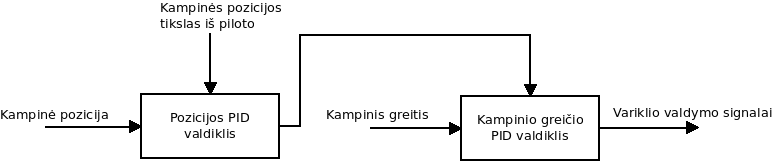
\includegraphics[width=1.0\textwidth]{img/PID-chaining.png}
\caption{Nuoseklus PID jungimas greičiui ir kampiniai pozicijai valdyti. PID valdikliai vaizduojami su rodykle iš kairės reiškiančią matuojamą proceso kintamąjį, iš viršaus tikslo kintamąjį, dešinėje -- PID išeitis.}
\label{pav-PID-series}
\end{center}
\end{figure}


\paragraph{PID paklaidos skaičiavimas}
Ketursraigčio kampinės padėties valdymui naudojami du valdikliai apibūdinti ankstesniame skyrelyje.
Vienas valdo sukimąsi apie lokalią $X$ ašį, valdydamas apie $Y$ ašį išdėliotus variklius, kitas valdo sukimąsi apie $Y$ ašį valdydamas apie $X$ ašį išdėliotus variklius.
Matuojamas proceso kintamasis yra kampas nuo horizontalios padėties.
O PID paklaida (ang.: \textit{error}) yra skirtumas tarp matuojamo kintamojo (kampo nuo horizontalios pozicijos) ir piloto (arba autopiloto) nustatytos reikšmės.

PID paklaidą skaičiuojama pagal $q_p$ kvaternioną (žr.: \ref{subskyr-final-quaternion})

Iš pradžių apskaičiuojamas aukštis, kuriame yra atitinkamas $X$ arba $Y$ variklis.
Tam sudaromas kvaternionas žymintis variklio poziciją lokalioje koordinačių sistemoje.

\begin{equation}
	q_{eng_x} = \left[
		\begin{array}{c}
			0 \\
			1 \\
			0 \\
			0
		\end{array}
	\right]
\end{equation}

Šis kvaternionas pasukamas pozicijos kvaternionu:

\begin{equation}
	q_{{eng_x}_h} = q_p * q_{eng_x} * q_p^{-1}
\end{equation}

Ir jo pozicija projektuojama į $Z$ ašį.

\begin{equation}
	h_x = q_{{{eng_x}_h}_z}
\end{equation}

Tuomet apskaičiuojamas kampas:

\begin{equation}
	\alpha = arcsin(h_x)
\end{equation}

$\alpha$ jau gali būti naudojamas kaip matuojamas proceso kintamasis pozicijos PID valdikliui, taip pat $\dfrac{d}{dt}\alpha$ naudojamas greičio PID valdikliui, tik diskretizuota versija:
\begin{equation}
	\dfrac{d}{dt}\alpha \widehat{=} \alpha_t - \alpha_{t-1}
\end{equation}


Verta pastebėti, kad šitoks skaičiavimas teisingai paklaidas skaičiuoja tik iki tol, kol jos neviršyja 90\degree, bet ketursraigtis negali išsilaikyti ore palinkęs tokiais stipriais kampais, todėl atvejai su tokiais kampais nėra nagrinėjami.

PID valdiklio išeitis yra naudojama modifikuoti dabartiniam galios tikslui (ang.: \textit{setpoint}), jeigu tai yra PID valdiklis valdantis pasisukimą pagal $X$ ašį, tuomet antram varikliui galia yra didinama tiek, kokia yra PID išeitis, o trečiam atitinkamai mažinama.
Analogiškai veikia ir $Y$ ašis.

\subsection{Pasisukimo pagal lokaliąją $Z$ ašį valdymas}

Ketursraigčių pasisukimas apie $Z$ ašį remiasi tuo, kad iš keturių propelerių du sukasi pagal ir du prieš laikrodžio rodyklę.
Oro pasipriešinimas sukelia jėgą verčiančią ketursraigtį suktis priešingą kryptimi negu propeleriai.
Kol bendras jėgų didumas propeleriams besisukantiems pagal laikrodžio rodyklę yra panašus į jėgų didumą propeleriams besisukandiems prieš laikrodžio rodyklę, tol šios jėgos viena kitą kompensuoja ir ketursraigtis nesisuka apie savo lokaliąją $Z$ ašį.
Pakeitus šį balansą galima priversti ketursraigtį suktis viena ar kita kryptimi, tačiau šia ašimi ketursraigčiai yra kur kas mažiau manevringesni negu $X$ ar $Y$ todėl valdymo algoritmas yra kur kas paprastesnis.

Kaip ir PID kontrolerio atveju, čia skaičiuojama pasisukimo pagal $Z$ ašies paklaida.

Sugeneruojamas kvaternionas atitinkantis $X$ variklio poziciją lokalioje koordinačių sistemoje.

\begin{equation}
	q_{eng_x} = \left[
		\begin{array}{c}
			0 \\
			1 \\
			0 \\
			0
		\end{array}
	\right]
\end{equation}

Pasukamas pagal esamą poziciją

\begin{equation}
	q_{{eng_x}_l} = q_p * q_{eng_x} * q_p^{-1}
\end{equation}

Čia imamas $X$, $Y$ vektorius ir normalizuojamas.

\begin{equation}
	x_{nenorm} = \left[
		\begin{array}{c}
			q_{{{eng_x}_l}_x} \\
			q_{{{eng_x}_l}_y}
		\end{array}
	\right]
\end{equation}

\begin{equation}
	x = \dfrac{x_{nenorm}}{||x_{nenorm}||}
\end{equation}

Ir skaičiuojamas kampas

\begin{equation}
	\alpha_z = \begin{cases}
		arccos(x_x), & \text{jeigu } x_y \geq 0\\
		-arccos(x_x), & \text{kitu atveju}
	\end{cases}
\end{equation}

Valdymo signalai yra gaunami: 
\begin{equation}
	u_z = \alpha_z * K_{p_z}
\end{equation}

Šis valdymo signalas yra pridedamas prie variklių galios besisukančių pagal laikrodžio rodyklę, ir atimamas iš variklių, besisukančių prieš laikrodžio rodyklę.




\section{Skrydžio autonomiškumas}
\label{skyr-autonomus}

Skrydžio autonomiškumas pasiekiamas atviro ciklo valdikliu, siunčiant valdymo komandas žemesniame valdymo lygmenyje esantiems PID valdikliams.

\subsection{Atviro-ciklo valdymas}

Atviro ciklo valdiklis tai yra valdiklis, kuris skaičiuoja valdymo parametrus tik pagal dabartinę būseną ir neatlieka valdomo objekto matavimų.
Šio tipo valdiklis ketursraigčiui buvo parinktas dėl fizinių sensorių nebuvimo, kurie galėtų matuoti ketursraigčio poziciją.

\subsection{Kampinės pozicijos tikslų lentelė}

Ketursraigčio valdymas atliekamas valdant bendrąją galią bei kampą pagal $X$, $Y$, $Z$ ašis.
Šiuos duomenis priima kampinės pozicijos valdikliai, kaip tikslo kintamuosius, ir nustato atitinkamas variklių galias.

Ketursraigčio valdymui sudaroma šių tikslų lentelė ir jie yra siunčiami ketursraigčiui periodiškai.

\begin{center}
\begin{table}[h]
\begin{tabular}{ | c | c | c | c | c | }
	\hline
	\textbf{galia} & \textbf{kampas $X$} & \textbf{kampas $Y$} & \textbf{kampas $Z$} & \textbf{galiojimo laikas} \\
	\hline
	20 \% & 0\degree & 0\degree & 0\degree & 2s \\
	\hline
	40 \% & 0\degree & 5\degree & 0\degree & 1s \\
	\hline
	40 \% & 0\degree & -5\degree & 0\degree & 1s \\
	\hline
	40 \% & -5\degree & 0\degree & 0\degree & 1s \\
	\hline
	40 \% & 5\degree & 0\degree & 0\degree & 1s \\
	\hline
	20 \% & 0\degree & 0\degree & 0\degree & 2s \\
	\hline
\end{tabular}
\caption{Supaprastintas tikslų lentelės pavyzdys}
\end{table}
\end{center}

Nepriklausomai nuo galiojimo laiko, tikslai yra siunčiami 10Hz dažniu, jeigu galiojimo laikas yra ilgesnis -- siunčiamas tas pats tikslas, kol galiojimo laikas pasibaigia.
Taip ketursraigtis turi galimybę atpažinti ar nenutrūko ryšys su pilotu ar pilotuojančia programa.

\subsection{Atviro-ciklo valdymo trūkumai}

Vertinant šį algoritmą pagal pozicijos paklaidas (lyginant du skrydžius vieną su kitu), yra labai didelės paklaidos dėl šio algoritmo nesugebėjimo prisitaikyti prie nenumatytų išorinių ir vidinių veiksnių (pvz.: Vėjo).
Taip pat PID valdikliai nėra tikslūs, o tai dar labiau padidina paklaidas.

TODO\_DIAGRAM\_OF\_ANGLE\_ERROR

TODO\_DISTURBANCE\_EXAMPLE


\section{Programinė įranga}
\label{skyr-software}
\subsection{Bendroji architektūra}

Ketursraigtis susideda iš trijų esminių fizinių dalių:
\begin{itemize}
	\item kompiuterio -- formuojančio ir siunčiančio valdymo komandas;
	\item retransmitoriaus -- persiunčiančio valdymo komandas ketursraigčiui;
	\item pagrindinės valdymo elektronikos -- valdančios ketursraigčio skrydį.
\end{itemize}

Kiekviena iš šių dalių turi savo programinę įrangą.

\subsection{Kompiuteriui skirtas klientas}

Kompiuteriui skirto kliento buvo paruoštos dvi versijos, viena skirta rankiniam ketursraigčio valdymui vairalazde, kita įgyvendinanti aptartą atviro ciklo valdymo algoritmą (žr.: \ref{skyr-autonomus}).

Abiejais atvejais tai yra "`python"' kalba parašyta programa, 10Hz dažniu nuskaitydama tikslo vertes (ar iš lentelės ar iš vairalazdės) ir suformuodama UDP paketą (žr.: pav. \ref{pav-ctrl-packet})

\begin{figure}[H]
\begin{center}
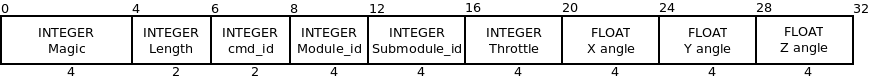
\includegraphics[width=1.0\textwidth]{img/ctrl_packet.png}
\caption{Valdymo paketas siunčiamas valdymo elektronikai. Skaičius apačioje rodo lauko dydį baitais, viršuje lauko poslinkį nuo paketo pradžios}
\label{pav-ctrl-packet}
\end{center}
\end{figure}



\subsection{Retransmitorius}

Retransmitorius kartu yra ir fizinis įrenginys.
Tai yra Raspberry Pi kompiuteris su Linux operacine sistema.
Šis kompiueris sukonfigūruotas prisijungti prie 3G/4G tinklų ir klausosi UDP paketų siunčiamų jo adresu.
Visą gautą informaciją jis tiesiog persiunčia per USB sąsają valdymo elektronikai.

\subsection{Ketursraigčio pagrindinis valdiklis}

Pagrindinės valdymo elektronika sudaro GY-86 sensorių plokštė, su giroskopu ir akselerometru, keturi vienetai greičio valdiklių, ir STM32F401 procesoriumi.
Iš šitų elementų vienintelis STM procesorius reikalauja programavimo, tad jam buvo parašyta programinė įranga įgyvendinanti visus sukurtus algoritmus ir vykdanti skrydžio kontrolę.
STM programinė įranga yra išskaidyta į modulius.

\begin{itemize}
	\item I2C -- modulis skirtas palaikyti komunikacijai su sensoriais.
	\item MPU6050 -- sensorių tvarkyklės modulis.
	\item Quaternion -- kvaternionų algebrą įgyveninantis modulis.
	\item IMU\_Horizon -- pozicijos kvaternioną skaičiuojantis modulis.
	\item AttitudeCtrl -- kampinės pozicijos valdymo modulis.
	\item PWM\_OUT -- modulis generuojantis signalą variklių valdikliams.
	\item Connection -- USB komandų palaikymo modulis.
	\item ConfigParam -- abstraktus konfiguracijos parametru modulis.
\end{itemize}


Verta pastebėti, kad kodas rašytas C kalba, bet šiek tiek mėgdžiojami kai kurie OOP principai.
Todėl toliau pateikiama klasių diagrama atitinkanti programinės įrangos struktūrą, jei ji būtų rašoma objektine programavimo kalba.

\begin{figure}[H]
\begin{center}
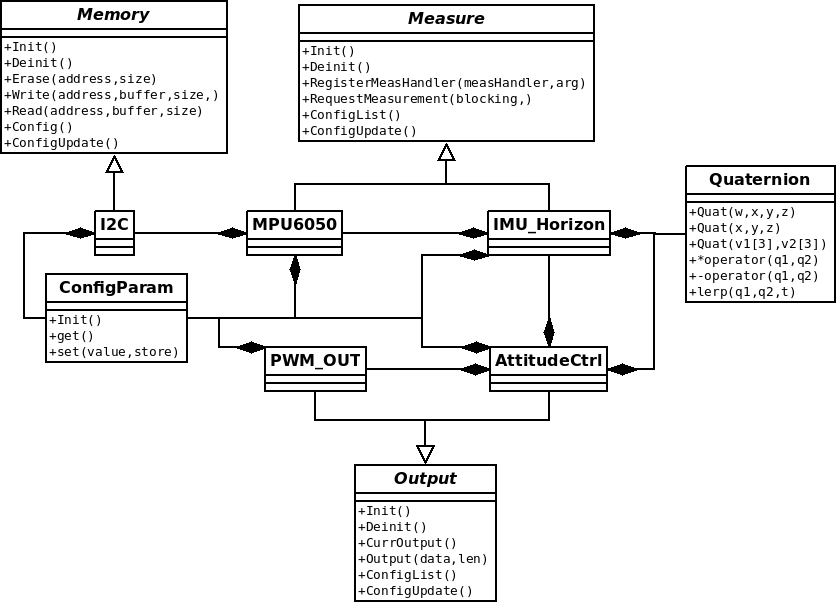
\includegraphics[width=0.9\textwidth]{img/classDiagram.png}
\caption{Vidinė pagrindinio valdiklio programinė struktūra.}
\end{center}
\end{figure}


\paragraph{"`Connection"' modulis}
"`Connection"' yra modulis, kuris jungiasi su visomis klasėmis, dėl to atskirai nebuvo pavaizduotas diagramoje.
Jis turi tik vieną "`Init"' metodą.
"`Connection"' modulis yra atsakingas už informacijos paėmimą iš USB sąsajos ir jos perdavimą atskiriems moduliams pagal jų ID.
Komunikacija per USB sąsają palaikoma pagal serverio-kliento principus.
Kompiuteris būdamas klientu siunčia užklausas ir sulaukia atsakymo kiekvienai užklausai.

"`Connection"' modulis palaiko šias komandas:
\begin{enumerate}
	\item \textit{Reset} -- perkrauna įrenginį;
	\item \textit{Enable device} -- aktyvuoja modulį;
	\item \textit{Disable device} -- deaktyvuoja modulį;
	\item \textit{SetConfig} -- nustato parametro reikšmę;
	\item \textit{ListActive} -- pateikia aktyvių modulių sąrašą;
	\item \textit{ListSupported} -- pateikia palaikomų modulių sąrašą;
	\item \textit{ListParam} -- pateikia konkretaus akyvaus modulio parametrų sąrašą;
	\item \textit{Output} -- iškviečia modulio, įgyvendinančio "`Output"' sąsają metodą "`Output"';
	\item \textit{CurrOutput} -- iškviečia modulio, įgyvendinančio "`Output"' sąsają metodą "`CurrOutput"';
	\item \textit{ListChecker} -- pateikia klaidų žurnalą;
	\item \textit{RequestMeasurement} -- iškviečia modulio, įgyvendinančio "`Measure"' sąsają metodą "`RequestMeasurement"'.
\end{enumerate}

Visos komandos paklusta baziniam protokolui, kuriame nurodomas komandos ilgis baitais, komandos identifikatorius be argumentai skirti konkrečiai komandai (žr.: pav. \ref{pav-cmd-proto}).

\begin{figure}[H]
\begin{center}
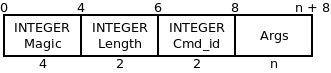
\includegraphics[width=0.5\textwidth]{img/basePacket.png}
\caption{Bazinė "`Connection"' modulio užklausos paketo struktūra. Skaičius viršuje rodo poslinkį nuo paketo pradžios, apačioje -- lauko ilgį.}
\label{pav-cmd-proto}
\end{center}
\end{figure}

Čia laukas "`Magic"' yra paketo pradžios identifikatorius ir visada įgauna tokią pačią reikšmę, kurį yra lygi A5B7C957 šešioliktainėje sistemoje.
Laukas "`Length"' nurodo viso paketo ilgį (įskaitant ir "`Magic"' bei "`Length"' laukus). Kiekviena komanda turi savo ID, kuris pateikiamas lauke "`Cmd\_id"', o lauke "`Args"' sudedama jau konkreti kiekvienos komandos reikalaujama informacija.






\vumifsectionnonum{Išvados}

Šiame darbe buvo sukurta fizikiniu modeliu besiremianti ketursraigčio skrydžio valdymo sistema, bei algoritmai, kuriais ši sistema vadovaujasi.


Darbe buvo išvestas supaprastintas fizikinis ketursraigčio skrydžio modelis, sukurtas kvaternionais grįstas algoritmas, leidžiantis rasti ketursraigčio kampinę poziciją, pasinaudojant nebrangiais MEMS giroskopo bei akselerometro sensoriais.
Toliau pritaikomi uždaro-ciklo PID algoritmai ketursraigčio kampinės pozicijos valdymui, taip pat pateikiamas atviro-ciklo valdymo algoritmas ketursraigčio pozicijos kontrolei.
Visa tai buvo suprogramuota ir išbandyta realaus ketursraigčio skrydžio metu.


\paragraph{Rezultatai}

Šiame darbe buvo sukurti bei išbandyti trys esminiai algoritmai: ketursraigčio kampinės pozicijos skaičiavimo, ketursraigčio kampinės pozicijos valdymo bei ketursaigčio pozicijos valdymo algoritmas.
Kampinės pozicijos algoritmas parodė gerus rezultatus, net ir sunkiomis darbo sąlygomis, kuomet sensoriai dirbo stiprios vibracijos sąlygomis.
Sensoriui dirbant normaliomis sąlygomis (vibracijų dažnis žemesnis nei ketvirtadalis matavimų dažnio, ir akseleracijos bei sukimo greičiai neviršyja sensoriaus matavimo ribų), buvo pasiekta mažesnė nei 1\degree paklaida, taip pat nebuvo aptikta jokių užrakinimo (ang.: \textit{gimbal lock}) pozicijų, būdingų panašiems algoritmams besiremiantiems oilerio kampais.
Tuo tarpu PID algoritmas parodė šiek tiek prastesnius rezultatus.
Esant mažoms kampinės pozicijos paklaidoms buvo pastebimas lengvas ketursraigčio kampinės padėties svyravimas.
Atviro ciklo pozicijos valdymas turėjo stiprias paklaidas, ir tiksliam autonominiam skrydžiui palaikyti -- reikėtų ieškoti kito algoritmo.


\paragraph{Tolimesni darbai, patobulinimai}

PID algoritmai nesuteikia optimalaus valdymo, ypač kai jų parametrai yra nustatomi rankiniu būdu ir randamas tik "`pakankamai-geras"' parametrų derinys.
Tuo tarpų tiesinis-kvadratinis reguliatorius (ang.: \textit{linear-quadratic regulator} arba \textit{LQG}), nors ir lieka šiek tiek rankinio algoritmo reguliavimo, teoriškai galėtų pasiekti geresnius rezultatus.
Taip pat specialūs fizika paremti modeliai valdymui galėtų būti sukurti agresyviam ketursraigčio valdymui.

Pozicijos valdymas galėtų būti išreikštas uždaro-ciklo valdymo algoritmu, įtaisius tikslius GPS įtaisus, sukūrus modelį bei algoritmus pozicijos valdymui.
Tokie patobulinimai pozicijos valdymo tikslumą galėtų pagerinti dešimtis ar net šimtus kartų.
Taip pat oro slėgio sensoriai galėtų būti naudojami automatiniam skrydžio aukščio valdymui.
Tam irgi turėtų būti sukurtas modelis, bei valdymo algoritmai.


TODO nuoroda
\bibliography{paper}

\end{document}



